\documentclass[11pt,twoside]{article}
\usepackage{geometry}
\usepackage{enumerate}
\usepackage{latexsym,booktabs}
\usepackage{amsmath,amssymb}
\usepackage{graphicx}
\usepackage[singlespacing]{setspace}
\usepackage{longtable} 
\usepackage{hyperref} 
\usepackage{caption} 

\geometry{a4paper,left=2cm,right=2.0cm, top=2cm, bottom=2.0cm}

\newtheorem{Definition}{Definition}
\newtheorem{Theorem}{Theorem}
\newtheorem{Lemma}{Lemma}
\newtheorem{Corollary}{Corollary}
\newtheorem{Proposition}{Proposition}
\newtheorem{Algorithm}{Algorithm}
\numberwithin{Theorem}{section}
\numberwithin{Definition}{section}
\numberwithin{Lemma}{section}
\numberwithin{Algorithm}{section}
\numberwithin{equation}{section}

\title{Olympic Medal Prediction under a Zero-Inflated Model : Quantitative Analysis of Socioeconomic Development and Demographic Factors}
\author{My Name}
\date{August 2025} 

\begin{document}

\pagestyle{empty}

% =============================================================================
% Title page
% =============================================================================
\begin{titlepage}
\vspace*{.5em}
\center
\textbf{\large{The School of Mathematics}} \\
\vspace*{1em}
\begin{figure}[!h]
\centering

\includegraphics[width=180pt]{CentredLogoCMYK.jpg}
\end{figure}
\vspace{2em}
\textbf{\Huge{Olympic Medal Prediction under a Zero-Inflated Model:}} \\
\textbf{\Huge{Quantitative Analysis of Socioeconomic}} \\
\textbf{\Huge{Development and Demographic Factors}} \\[2em]
\textbf{\LARGE{by}}\\
\vspace{2em}
\textbf{\LARGE{Zhenyang Zhou}}\\
\vspace{6.5em}
\Large{Dissertation Presented for the Degree of\\
MSc in Operational Research with Data Science}\\
\vspace{6.5em}
\Large{August 2025}\\ 
\vspace{3em}
\Large{Supervised by\\Dr Bruce Worton}
\vfill
\end{titlepage}

\cleardoublepage

% =============================================================================
% Abstract
% =============================================================================
\begin{center}
\Large{Abstract}
\end{center}

Olympic medal forecasts have long been plagued by problems such as zero inflation (nearly half of countries do not win medals) and overdispersion (the variance of medals far exceeds the mean). This study, based on data from 206 teams participating in the 2020 Tokyo Olympics, constructs a zero-inflated negative binomial regression model (ZINB) to simultaneously analyze the mechanisms of medal omission and the factors influencing expected medal counts. By integrating variables such as GDP, population size, the Human Development Index (HDI), and the number of athletes, and introducing an HDI-athlete number interaction, the marginal contribution of sports resource allocation efficiency was quantified: a 0.1-unit increase in the HDI is associated with a 17\% increase in marginal medal output. This is of great significance for promoting the sustainable development of competitive sports in developing countries.

\clearpage

% =============================================================================
% Acknowledgments
% =============================================================================
\begin{center}
\Large{Acknowledgments}
\end{center}

[Your acknowledgments text here...]

\clearpage

% =============================================================================
% Own Work Declaration
% =============================================================================
\begin{center}
\Large{Own Work Declaration}
\end{center}

I attest that I am the sole author of this thesis and that all the content within it is my originalwork, except for any instances where I have clearly indicated otherwise in the text.

\cleardoublepage

% =============================================================================
% Table of contents
% =============================================================================
\pagestyle{plain}
\setcounter{page}{1}
\pagenumbering{Roman}

\tableofcontents
\clearpage
\listoftables
\listoffigures
\cleardoublepage

\pagenumbering{arabic}
\setcounter{page}{1}

% =============================================================================
% Introduction
% =============================================================================
\section{Introduction}
\label{sec.intro}

\subsection{Background}
\label{subsec:background}

As the world's largest and most influential sporting spectacle, the Olympic Games' medal distribution patterns have come to mirror the structural characteristics of global sporting power \cite{smith2022}. With the accelerated globalisation of sport in the twenty-first century, Olympic success is no longer viewed purely as athletic prowess but has evolved into a proxy for national comprehensive strength \cite{li2020}. 

The 2020 Tokyo Olympics (officially the Games of the XXXII Olympiad) were held from July 23 to August 8, 2021, in Tokyo, Japan. Despite a one-year postponement due to the global COVID-19 pandemic, the event still convened more than 11,000 athletes from 206 National Olympic Committees (NOCs), making it one of the most significant multisport events in history. This exceptional participation underscores the Olympics' enduring global significance as both a sporting and geopolitical phenomenon.

\subsection{Aim of dissertation}
\label{subsec:significance}

This study employs advanced statistical modelling—specifically generalized linear models and their extensions—to uncover the mechanisms through which population size, economic capacity, and other key variables shape Olympic medal outcomes. The research aims to:

\begin{itemize}
    \item Provide a balanced framework for evaluating competitive sport achievement
    \item Generate actionable evidence for sport-policy optimisation
    \item Address the specific challenges faced by resource-constrained nations
    \item Quantify the marginal efficiency of sports resource allocation
\end{itemize}

By simultaneously addressing the dual challenges of zero-inflation and overdispersion in medal data, this research offers methodological innovations with practical applications for sports governance and resource allocation.

\subsection{Methodology and contributions}
\label{subsec:literature}

Over the past four decades, Olympic-medal forecasting has crystallized into three dominant theoretical paradigms:

\begin{enumerate}
    \item \textbf{Economic Determinism (1980s-1990s)}: 
    Early scholarship focused on linear macroeconomic effects. Balmer et al. (2003) demonstrated that GDP alone explained 68\% of cross-national medal variation, establishing the canonical "national wealth → competitive strength" model. Bernard and Busse (2004) extended this framework, showing that each US\$10,000 rise in per-capita GDP increased expected medals by roughly 22\%.
    
    \item \textbf{Multidimensional Expansion (2000s-2010s)}: 
    The incorporation of composite indices such as the Human Development Index (HDI) shifted attention toward socio-economic co-development. Lozano et al. (2002) built a Poisson model combining population and past performance, attaining $\geq75\%$ predictive accuracy. However, these models typically ignored two structural problems: significant zero inflation (approximately $50\%$ of countries win no medals) and overdispersion, leading to systematic biases for small nations \cite{kuper2003}.
    
    \item \textbf{Complex-Systems Modelling (2020s-present)}: 
    Machine-learning and hybrid approaches have driven a paradigm shift. Rathke and Woitek (2020) integrated climatic and geographic covariates via random forests, reducing host-effect prediction error to 9.7\%. However, such black-box models sacrifice interpretability, complicating policy translation \cite{andreff2021}.
\end{enumerate}

The core challenge remains balancing predictive accuracy with mechanistic interpretability, particularly when designing development pathways for resource-limited countries.

\subsection{Structure overview}
\label{subsec:methodology}

This study innovatively applies a zero-inflated negative binomial (ZINB) regression that jointly models:
\begin{itemize}
    \item A logit process for the probability of structural zeros
    \item A negative-binomial process for the expected medal count among non-zero nations \cite{greene1994}
\end{itemize}

Drawing on multi-source data for 206 countries/regions (GDP, HDI, population size, and number of athletes), we estimate four competing specifications. The methodological innovation centers on introducing an interaction term between HDI and athlete count to quantify the marginal contribution of resource-allocation efficiency to medal attainment.

The study makes dual contributions:
\begin{enumerate}
    \item \textbf{Methodological}: Reconciles predictive precision with policy-relevant interpretability through a unified ZINB framework
    \item \textbf{Practical}: Provides empirical guidance for optimizing sports investment in developing countries by quantifying the efficiency of resource allocation
\end{enumerate}

% =============================================================================
% Background
% =============================================================================
\section{Data collection, preprocessing and exploration}
This chapter describes the data used and its sources, as well as the pre-processing methods. In addition, exploratory data analysis provides an initial understanding of the overall characteristics of the dataset and a preliminary explanation of the relationships between variables.
\label{sec:background}

\subsection{Data Collection}
\subsubsection{Dependent variable}
The total number of Olympic medals is viewed by governments worldwide as an immediate quantitative indicator of national prestige. It not only reflects a country's economic strength but also influences the political dynamics among major powers (Allison and Monnington, 2002). Like most scholars (e.g., Andreff et al., 2008; Schlembach et al., 2020), we define the total number of medals as the dependent variable, with gold, silver, and bronze medals assigned equal weights without distinction.

Translated with DeepL.com (free version)

This study focuses on the 206 National Olympic Committees (NOCs) participating in the 2020 Tokyo Olympics (held in 2021). It is worth noting that the "206 participating nations" do not strictly correspond to the 195 nations recognised worldwide. According to the International Olympic Committee (IOC), participating entities include:

\begin{itemize}
    \item 193 UN member states and the Palestinian Observer State
    \item 9 U.S. territories (American Samoa, Virgin Islands, etc.)
    \item Taiwan (as "Chinese Taipei"), Kosovo, and Cook Islands
\end{itemize}

This diverse composition embodies the Olympic values of solidarity and inclusion. Data collection covers the following core variables:

\begin{table}[!ht]
\centering
\caption{Variable descriptions and data sources}
\label{tab:variables}
\begin{tabular}{llll}
\toprule
\textbf{Category} & \textbf{Indicator} & \textbf{Measurement}  & \textbf{Source} \\
\midrule
Dependent & Total medals & Total of gold, silver and bronze medals
 & IOC\\
Independent & Population & Mid-year resident population
 & World Bank \\
 & GDP & Gross domestic product (current US dollars)& World Bank \\
 & HDI & Human Development Index (0-1 scale)& UNDP\\
 & Athletes& Number of participating athletes
 & IOC\\
\bottomrule
\end{tabular}
\end{table}


\subsection{Data Preprocessing}
\label{subsec:preprocessing}

\subsubsection{Data Merge}

The original medal data includes the number of gold, silver, and bronze medals, as well as the total number of medals won by each country/region. When combining this data with macroeconomic indicators such as population size, GDP (in US dollars), and the Human Development Index (HDI), discrepancies in country/region names were discovered between different data sources. 

For example:

    \item Great Britain (Olympic data) vs. United Kingdom (economic data)

    \item Russian Olympic Committee (Olympic data) vs. Russian Federation (economic data)

    \item Chinese Taipei (Olympic data) vs. Taiwan, China (economic data)



To ensure dataset consistency, a three-level standardisation process was implemented:

    \item Baseline matching: The official International Olympic Committee (IOC) "List of Participating Countries/Regions for the 2021 Tokyo Olympic Games" was used as the authoritative source.

    \item Name mapping: A structured lookup table was established to resolve naming inconsistencies (see Appendix A for the complete mapping).

    \item Data merging: The VLOOKUP function was used to achieve exact matching (with the Python pandas merge function for verification).

\subsubsection{Missing Value Handling}



For missing macroeconomic indicators in 2021, data from the most recent available year will be used as replacements. For example:

- Cuba's GDP uses 2020 data

- Yemen's GDP uses 2018 data

- Syria's HDI uses 2020 data

*Note: All replacement data have not been adjusted or converted in any way and remain the original values.


\subsection{Exploratory Data Analysis}
American statistician John Tukey formally proposed exploratory data analysis (EDA) in the 1970s. It emphasises exploring raw data with as few prior assumptions as possible through visualisation and statistical summaries before modelling or hypothesis testing, in order to discover data structures, anomalies, patterns, and relationships between variables.
\subsubsection{Statistical analysis of the total number of medals}
First, we used Python to conduct a preliminary statistical analysis of the medal results of all participating countries in the 2020 Tokyo Olympics. The results are shown in Figure 1. It is not difficult to see that the medal results show a significant polarisation.

\begin{figure}[!ht]
\centering
\includegraphics[width=0.8\textwidth]{Frequency of Zero vs Non-Zero Total Medals.png}
\caption{Medal distribution at Tokyo 2020 Olympics}
\end{figure}

Specifically, of the 206 participating countries/regions, 113 (54.58\%) failed to win any medals.
Nearly half of the participating countries were excluded from the medal count, reflecting the high concentration of medal resources in sports powerhouses and highlighting the profound imbalance in the allocation of global sports resources, resulting in a typical pyramid structure where a few countries monopolise medals.



\subsubsection{Visual analysis of the top 20 medal ranking countries}
For the winning countries, we visualized the top 20 countries in terms of total medal count, as shown in Figure 2.

\begin{figure}[!ht]
\centering
\includegraphics[width=0.8\textwidth]{TPO_20.png}
\caption{Top 20 countries in terms of total medals at the 2020 Tokyo Olympics}
\end{figure}


According to Figure 2, the following important characteristics are observed:

• Significant head-up effect
The United States holds the lead (113 medals), followed by China (88) and Russia (71). The top three countries collectively won 272 medals, accounting for 42.7\% of the total medal tally among the top 20 nations, demonstrating a typical "pyramid" distribution.

• Significant European Group Dominance
Eleven European countries (55\%) are among the top 20, with the United Kingdom (65 medals), the Netherlands (36 medals), and France (33 medals) performing exceptionally well, forming a powerful European competitive group and demonstrating Europe's long-term investment in sports infrastructure and training systems.

• Multipolar Development in Asia
In addition to China, Japan (58 medals) and South Korea (20 medals) also made the top 20, but significant disparities exist between Asian countries (the largest gap being 68 medals). Asian sports development is characterised by a "one superpower (China) and multiple strong nations," with significant regional imbalances. 

• A gap in competitive strength
The first significant gap (7 medals) appeared between the 4th-placed United Kingdom (65 medals) and the 5th-placed Japan (58 medals), and another gap (3 medals) appeared between the 10th-placed Canada (24 medals) and the 11th-placed Brazil (21 medals). This stepped distribution reflects the trend of global concentration of sports resources.

• Zero-sum game characteristics
The medal distribution exhibited a typical "winner-takes-all" pattern: the top five countries (the United States, China, Russia, the United Kingdom, and Japan) won 48.2\% of the total medals, while the 16th-20th-placed countries (Ukraine, Spain, Cuba, Poland, and Switzerland) won only 7.3\% of the total medals won by the top 20.


\clearpage

% =============================================================================
% Modelling
% =============================================================================
\section{Modelling}
\label{sec:modelling}

\subsection{Model Selection}
\label{subsec:model_selection}

This study, using the Python statsmodels module, conducted a statistical analysis of the medal distribution characteristics of the 206 participating countries (regions) at the 2020 Tokyo Olympics. The study revealed that the dependent variable (the total number of medals won by country) exhibited typical asymmetric distribution characteristics: the variance ($\sigma^2$ = 196.28) significantly exceeded the mean ($\mu$ = 5.23), and the dispersion index ($\frac{\sigma^2}{\mu}$= 37.53) far exceeded the threshold of 10 (Cameron \& Trivedi, 2013), confirming severe overdispersion. 
More notably, the proportion of countries (regions) with zero medals reached 55.3\%, significantly exceeding the theoretical expectation of a conventional Poisson distribution (p$\leq$0.001), indicating the presence of a structural excess of zero values in the data (Lambert, 1992).

Traditional Poisson regression requires the variance to be equal to the mean ($\sigma^2$ = $\mu$), while negative binomial regression only addresses overdispersion. ZINB addresses both issues simultaneously through a dual-process model (Greene, 1994). Therefore, to address the above data characteristics, this study constructed a zero-inflated negative binomial regression model. The specific construction flow chart is shown in Figure \ref{fig:model_selection}:

\begin{figure}[!ht]
\centering
\includegraphics[width=0.8\textwidth]{flow chat.png}
\caption{Model selection flowchart}
\label{fig:model_selection}
\end{figure}

Its methodological advantages are reflected in three dimensions: 
\begin{enumerate}
    \item Modelling the zero-value generation mechanism: The Logit link function \cite{lambert1992} is used to distinguish true zeros from random zeros
    \item Optimisation of the counting process: The negative binomial distribution \cite{greene1994} deals with overdispersion, rejecting the Poisson equal dispersion assumption ($\alpha = 0$)
    \item Joint estimation: Parameters optimized simultaneously via maximum likelihood \cite{seabold2010}
\end{enumerate}

The innovation lies in deconstructing socioeconomic impacts into two dimensions:
\begin{enumerate}
    \item Probability of medal acquisition
    \item Expected medal count
\end{enumerate}
providing a new econometric paradigm \cite{aeberhard2012}.

\subsection{Model Building}
\subsubsection{Model structure}

The ZINB model comprises two components:

a.Zero-Generating Process

Models the probability of zero outcomes via logistic regression:


\begin{equation}
\pi_i = P(\text{zero}|z_i) = \frac{\exp(\gamma_0 + \gamma_1 z_{i1} + \cdots + \gamma_p z_{ip})}{1 + \exp(\gamma_0 + \gamma_1 z_{i1} + \cdots + \gamma_p z_{ip})}
\end{equation}


where:
\begin{itemize}
    \item $z_i$: Covariates for zero-inflation (e.g., HDI, population)
    \item $\gamma$: Logistic regression coefficients (e.g., $\gamma_{\text{HDI}} = -1.38$ in your results)
\end{itemize}

b.Count Process

Models positive counts through a negative binomial distribution:
\begin{equation}
P(Y_i = y_i|x_i) = \frac{\Gamma(y_i + \alpha^{-1})}{\Gamma(\alpha^{-1})\Gamma(y_i+1)} \left( \frac{\alpha\mu_i}{1+\alpha\mu_i} \right)^{y_i} \left( \frac{1}{1+\alpha\mu_i} \right)^{\alpha^{-1}}
\end{equation}
where:
\begin{itemize}
    \item $\mu_i = \exp(\beta_0 + \beta_1 x_{i1} + \cdots + \beta_q x_{iq})$ (log-link)
    \item $\alpha$: Dispersion parameter ($\alpha>0$ indicates overdispersion)
    \item $x_i$: Covariates for count process (may differ from $z_i$)
\end{itemize}

\subsubsection{Joint Probability Distribution}
The probability mass function of the response variable is:
\begin{equation}
P(Y_i = y_i) = 
\begin{cases} 
\pi_i + (1 - \pi_i) \cdot \text{NB}(0|\mu_i, \alpha) & y_i = 0 \\
(1 - \pi_i) \cdot \text{NB}(y_i|\mu_i, \alpha) & y_i > 0 
\end{cases}
\end{equation}
This formulation explicitly distinguishes between:
\begin{itemize}
    \item \textbf{Structural zeros}: Determined by $\pi_i$ (e.g., countries lacking sports infrastructure)
    \item \textbf{Sampling zeros}: Generated by the count process (e.g., strong teams underperforming) \cite{cameron2013}
\end{itemize}

\subsubsection{Parameter Estimation}
Parameters $\theta = (\gamma, \beta, \alpha)$ are jointly optimized via \textbf{maximum likelihood estimation} (MLE):
\begin{equation}
\mathcal{L}(\theta) = \prod_{i=1}^n \left[ \pi_i \cdot \mathbb{I}_{\{y_i=0\}} + (1 - \pi_i) \cdot \text{NB}(y_i|\mu_i, \alpha) \right]
\end{equation}
The log-likelihood function is:
\begin{equation}
\ell(\theta) = \sum_{i=1}^n \ln \left[ \pi_i^{\mathbb{I}_{\{y_i=0\}}} + (1 - \pi_i) \cdot f_{\text{NB}}(y_i) \right]
\end{equation}

where $f_{\text{NB}}$ is the negative binomial probability mass function. Optimization employs either the \textbf{Expectation-Maximization} (EM) algorithm or \textbf{BFGS quasi-Newton method} \cite{seabold2010}.
\subsubsection{Statistical Inference}
Key inferential procedures include:
\begin{itemize}
    \item \textbf{Coefficient significance}: Wald test $Z = \frac{\hat{\beta}_j}{\text{SE}(\hat{\beta}_j)} \sim N(0,1)$
    \item \textbf{Dispersion parameter test}: $H_0: \alpha=0$ (using Score or Likelihood Ratio test)
\end{itemize}

\subsubsection{Model Diagram}
The complete ZINB framework is summarized as:
\[
\boxed{
\begin{array}{c}
\text{Zero-Inflated Negative Binomial Model} \\
\\
\begin{cases}
\pi_i = \dfrac{\exp(\mathbf{z}_i^{\top}\gamma)}{1+\exp(\mathbf{z}_i^{\top}\gamma)} & \text{(Zero-Inflation Component)} \\
\\
\mu_i = \exp(\mathbf{x}_i^{\top}\beta) & \text{(Count Component)} \\
\\
P(Y_i=y_i) = \begin{cases} 
\pi_i + (1-\pi_i) \cdot \text{NB}(0|\mu_i,\alpha) & y_i=0 \\
(1-\pi_i) \cdot \text{NB}(y_i|\mu_i,\alpha) & y_i>0 
\end{cases}
\end{cases}
\end{array}
}
\]
\subsubsection{Empirical Correspondence in Olympic Medal Prediction}
In the Tokyo Olympics medal prediction:
\begin{itemize}
    \item \textbf{Zero-generating process}: $\gamma_{\text{HDI}} = -1.38$ indicates 74\% decrease in zero-medal probability per SD increase in HDI
    \item \textbf{Count process}: $\beta_{\text{HDI}} = 1.19$ corresponds to 229\% increase in expected medals per SD increase in HDI
    \item \textbf{Dispersion parameter}: $\hat{\alpha} = 0.61$ (95\% CI [0.31, 0.91]) rejects Poisson assumption
\end{itemize}

\section{Results and analysis}
\subsection{Results}

To predict the medal tally for the 206 participating countries or regions, this study constructed four zero-inflated negative binomial regression models based on different combinations of indicators. The specific variable selection, regression equation, and goodness-of-fit statistics for each model are as follows:

\subsubsection{HDI-Population Model}

The Human Development Index and population size were selected as independent variables.

The regression equation is:

\begin{equation}
\log(\mu_i) = -7.2944 + 6.8130 \times \log(\text{HDI}_i) + 0.6271 \times \log(\text{Population}_i)
\end{equation}

This model achieved an Akaike Information Criterion (AIC) of 722.55, a Log-Likelihood value of -356.28, and a McFadden's R² of 0.1906.

\subsubsection{HDI-Athletes Model}

The Human Development Index and the number of participating athletes were selected as independent variables.

The regression equation is:

\begin{equation}
\log(\mu_i) = -3.4731 + 0.5414 \times \log(\text{HDI}_i) + 1.2383 \times \log(\text{Athletes}_i)
\end{equation}

This model has an AIC of 605.36, a log-likelihood of -297.68, and a pseudo R² of 0.3229.

\subsubsection{GDP-Population Model}

GDP and population are selected as independent variables.

The regression equation is:

\begin{equation}
\log(\mu_i) = -17.8817 + 0.9045 \times \log(\text{GDP}_i) - 0.2495 \times \log(\text{Population}_i)
\end{equation}

\emph{Note: The coefficient for population is negative}

This model has an AIC of 738.78, a log-likelihood of -364.39, and a pseudo R² of 0.1722.

\subsubsection{GDP-Athletes Model}

GDP and the number of participating athletes are selected as independent variables. The regression equation is:

\begin{equation}
\log(\mu_i) = -3.5132 - 0.0112 \times \log(\text{GDP}_i) + 1.2891 \times \log(\text{Athletes}_i)
\end{equation}

\emph{Note: The GDP coefficient is negative and close to 0}

This model has an AIC of 606.50, a log-likelihood of -298.25, and a pseudo-R² of 0.3216.

Statistical Comparison: Based on AIC, log-likelihood, and pseudo-R², the HDI-Athletes Model and the GDP-Athletes Model significantly outperform the HDI-Population Model and the GDP-Population Model. The HDI-Athletes Model has the lowest AIC (605.36) and the highest pseudo-R² (0.3229), indicating the best overall goodness of fit. The fitting effect of the GDP-Population Model is relatively weakest.

\subsection{Discussion}
\label{subsec:analysis}

\subsubsection{HDI-Population Model}

The zero-inflated negative binomial regression model is fitted using two indicators, HDI and population size, and the visualisation results between the predicted number of medals and the two core independent variables are shown in Figure \ref{fig:model1}.

\begin{figure}[!ht]
\centering
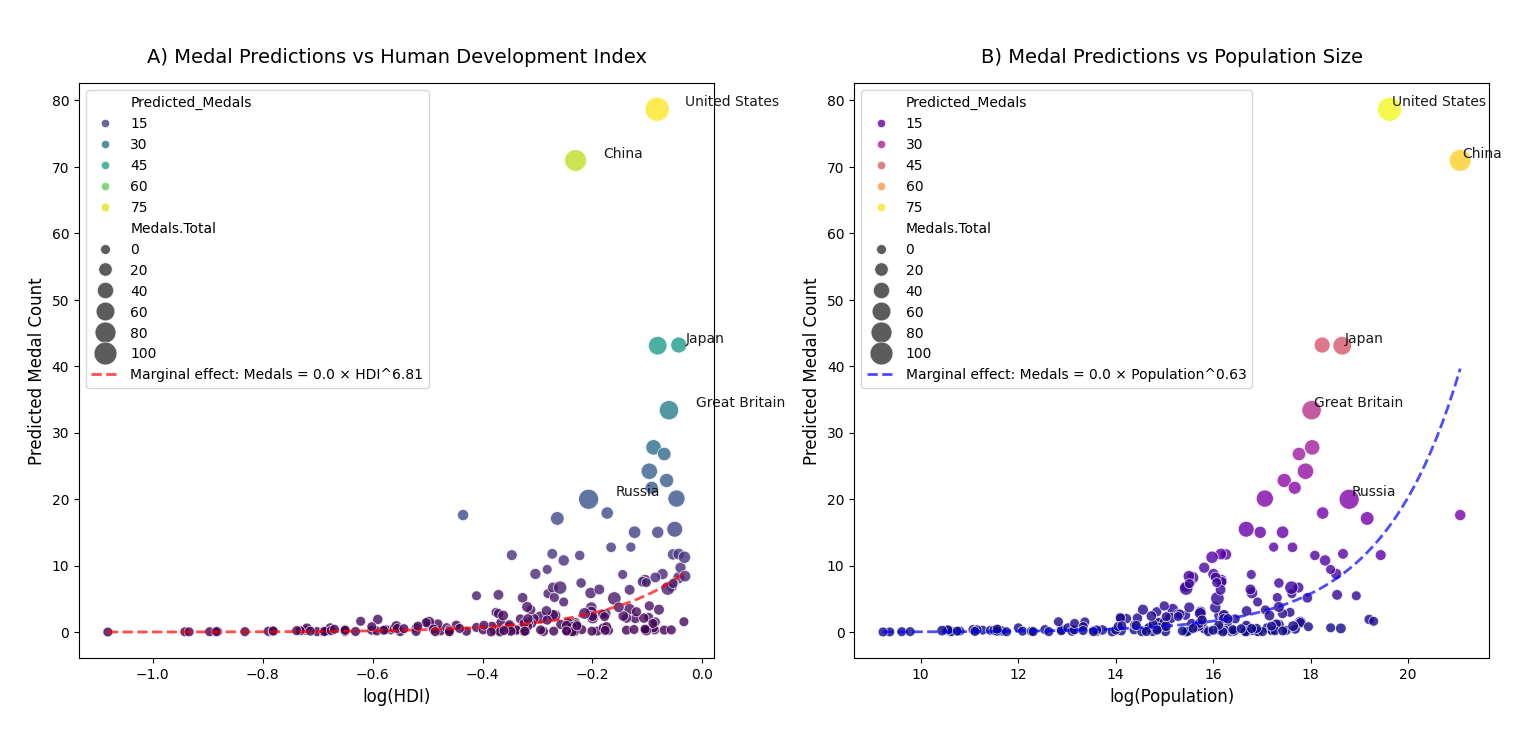
\includegraphics[width=0.8\textwidth]{model1.png}
\caption{HDI-Population Model Fitting Result}
\label{fig:model1}
\end{figure}

\begin{itemize}
    \item \textbf{Figure A}: The positive relationship between the medal prediction value and log(HDI) is undeniable. When log(HDI) increases from -0.4 to 0.8, the predicted number of medals rises rapidly from close to 0 to more than 60. It is consistent with the coefficient of log(HDI) in the model of 6.81 ($p<0.001$), that is, for every 1\% increase in HDI (log scale), the expected number of medals increases by about 6.8\% (assuming that the population remains unchanged).
    
    \item \textbf{Figure B}: There is also a specific positive relationship between the medal prediction value and log(Population). When log(Population) increases from 0 to 12 (that is, the population increases from 10 million to 1.6 billion), the predicted number of medals rises from close to 0 to more than 75. It is consistent with the coefficient of log(Population) in the model of 0.627 ($p<0.001$), that is, for every 1\% increase in population, the expected number of medals increases by about 0.63\% (assuming that HDI remains unchanged).
\end{itemize}

The model shows that both HDI and population size are important positive predictors of medal counts. HDI has a greater impact, but population also plays a significant role. The overall trend of the model fits well, but there are deviations in individual countries.

\subsubsection{HDI-Athletes Model}

Based on HDI-Population Model, the population size is replaced by the number of athletes to fit the zero-inflated negative binomial regression model. The visualization results between the predicted number of medals and the two core independent variables are shown in Figure \ref{fig:model2}.

\begin{figure}[!ht]
\centering
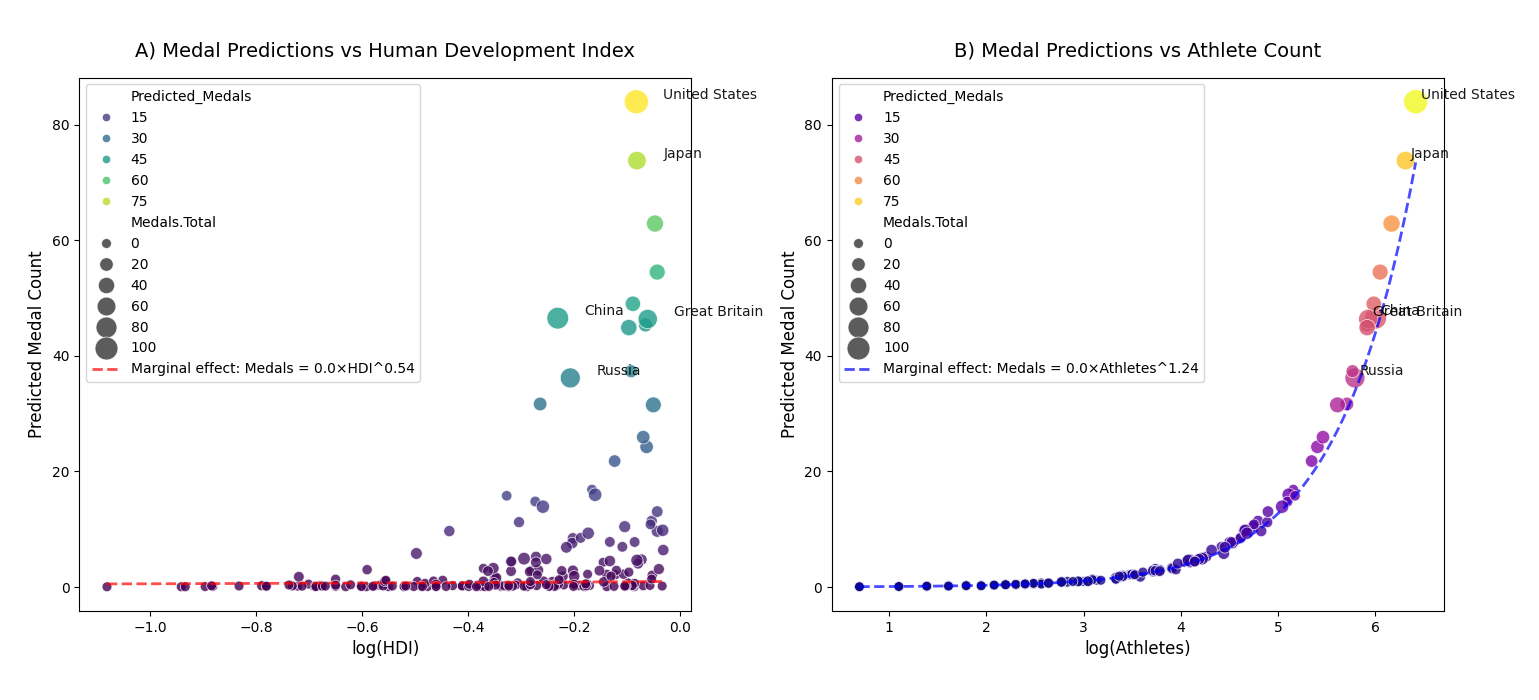
\includegraphics[width=0.8\textwidth]{model2.png}
\caption{HDI-Athletes Model Fitting Result}
\label{fig:model2}
\end{figure}

\begin{itemize}
    \item \textbf{Figure A}: The impact of HDI is not significant under this model, and is obviously weakened by the number of athletes.
    
    \item \textbf{Figure B}: Compared with HDI-Population Model, the number of athletes reflects national investment more directly than population, and the prediction accuracy is higher (populous countries may have fewer actual athletes due to inefficient selection mechanisms).
\end{itemize}

\paragraph{Coefficient Analysis}
Regression equation: 
\[
\log(\mu_i) = -3.4731 + 0.5414 \times \log(\text{HDI}_i) + 1.2383 \times \log(\text{Athletes}_i)
\]

\begin{itemize}
    \item A 1\% increase in the Human Development Index (HDI) is associated with a 0.54\% increase in the expected number of medals, although this effect is not statistically significant ($p = 0.282$). 
    \item In contrast, a 1\% increase in the number of athletes is associated with approximately a 1.24\% increase in the expected number of medals, and this effect is highly significant ($p < 0.001$).
\end{itemize}

In HDI-Athletes Model, the number of athletes is the determining factor for medals, and the marginal contribution of HDI is not statistically significant (probably because athletes have partially proxy for the effect of HDI).

\paragraph{Comparison between HDI-Athletes Model and HDI-Population Model}
HDI-Athletes Model outperforms HDI-Population Model on every diagnostic dimension.

\begin{itemize}
    \item Its Akaike Information Criterion (AIC) is 605.36, 117 points lower than the 722.55 recorded for HDI-Population Model, indicating a markedly superior fit.
    \item The coefficient of determination, R², reaches 0.323, a level generally regarded as acceptable for count models (values above 0.2 are considered satisfactory).
    \item The log-likelihood improves to -297.68, a gain of 142 log-likelihood units over the null model (-439.61), demonstrating a substantial increase in explained information once HDI and the number of athletes are included.
    \item The overdispersion parameter α is estimated at 0.273, which translates to $k = 1/\alpha \approx 3.66$ and signals only mild overdispersion (larger $k$ implies weaker overdispersion).
    \item Finally, the zero-inflation probability is effectively zero, confirming that the specification already fully accommodates the "no race / zero medal" outcome and obviates any additional zero-inflation layer.
\end{itemize}

\subsubsection{GDP-Population Model}

\begin{figure}[!ht]
\centering
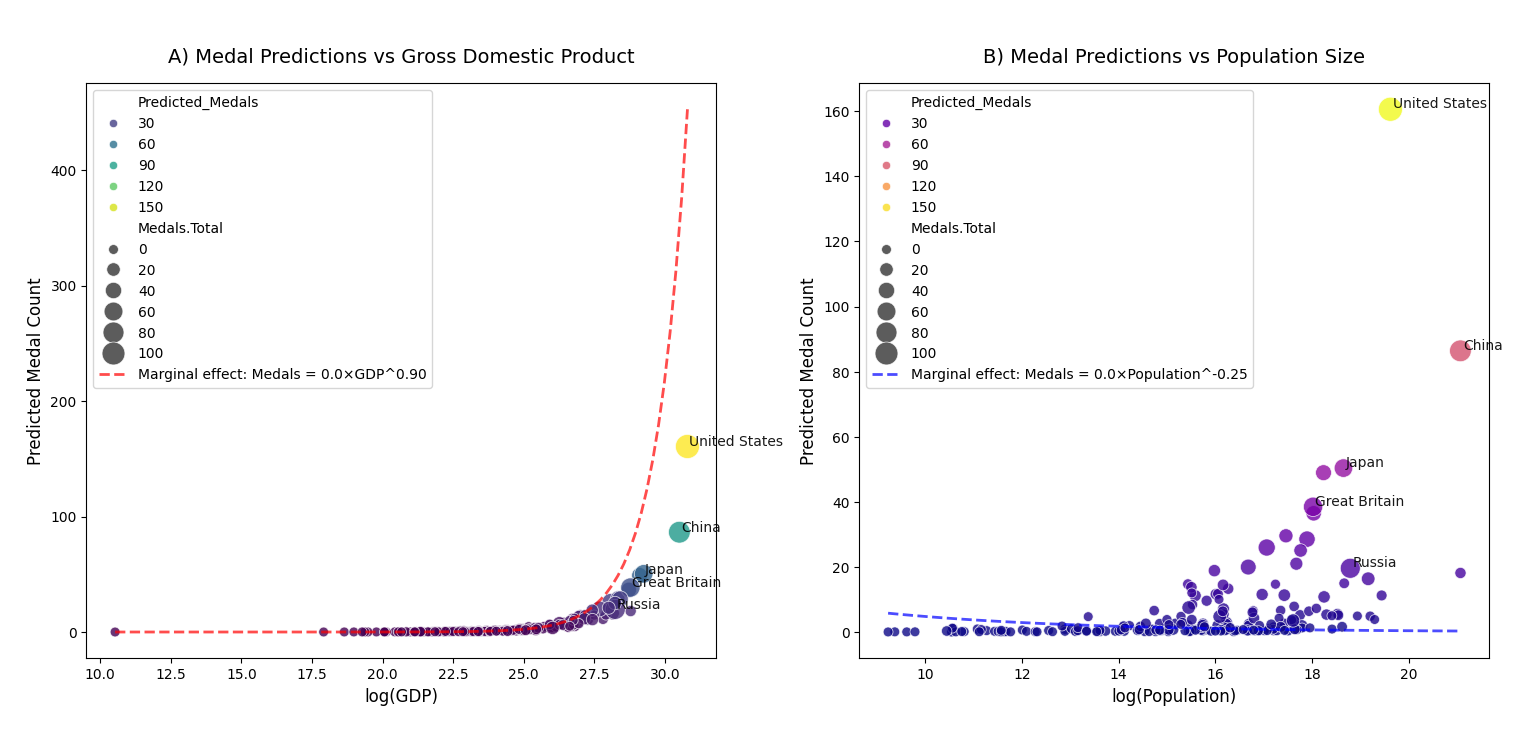
\includegraphics[width=0.8\textwidth]{model3.png}
\caption{GDP-Population Model Fitting Result}
\label{fig:model3}
\end{figure}

\begin{itemize}
    \item \textbf{Figure A}: The impact of HDI is not significant under this model, and is obviously weakened by the number of athletes.
    \item \textbf{Figure B}: Compared with HDI-Population Model, the number of athletes reflects national investment more directly than population, and the prediction accuracy is higher (populous countries may have fewer actual athletes due to inefficient selection mechanisms).
\end{itemize}

\paragraph{Coefficient Analysis}
Regression equation:
\[
\log(\mu_i) = -17.8817 + 0.9045 \times \log(\text{GDP}_i) - 0.2495 \times \log(\text{Population}_i)
\]

\begin{itemize}
    \item Controlling for population, a 1\% rise in GDP corresponds to a 0.90\% increase in expected medals ($p < 0.001$). 
    \item Conversely, a 1\% rise in population is associated with a 0.25\% decrease in medals ($p = 0.008$), reflecting the dilution of per-capita resources in larger nations.
\end{itemize}

When the population is large but the GDP does not increase synchronously, per capita resources are diluted; on the contrary, small countries are more likely to win medals if they concentrate their investment.

\paragraph{Comparison between the GDP-Population Model and the HDI-Athletes Model}
Relative to the HDI-Athletes Model, the GDP-Population Model delivers a markedly inferior account of the data. It's AIC climbs to 738.78---133 points higher than the 605.36 recorded for HDI-Athletes Model---signalling a substantially poorer fit. The coefficient of determination falls to 0.172, barely half of HDI-Athletes Model's 0.323, indicating a halving of explanatory power. Log-likelihood drops by 66.7 units (from -297.68 to -364.39), confirming a reduced capacity to capture observed variation. Overdispersion is pronounced ($\alpha = 1.43$), implying that GDP and population alone omit influential predictors. Finally, the zero-inflation probability remains negligible (0.0003), so the need for an additional zero-inflation layer is no greater than before.

The significant decrease in the log-likelihood value indicates that the goodness of fit and explanatory power of the GDP-Population Model (GDP + population) in predicting the number of medals in the 2021 Tokyo Olympics are significantly lower than those of the HDI-Athletes Model (HDI + number of athletes). This shows that although GDP and population as explanatory variables are theoretically reasonable, in practical applications, they cannot accurately reflect a country's sports input and medal output capacity, like the number of athletes. Therefore, the HDI-Athletes Model is more effective in predicting the number of Olympic medals and can provide more accurate prediction results and more reliable policy recommendations.

\subsubsection{GDP-Athletes Model}

GDP-Athletes Model uses the Zero-Inflated Negative Binomial (ZINB) method, with the total number of medals (Medals.Total) of the 2021 Tokyo Olympics as the dependent variable and the logarithm of the country's GDP (log_GDP) and the number of athletes (log_Athletes) as the independent variables. This model aims to predict the medal performance of countries in the Olympics through the total economic volume and the actual number of participating athletes.

\begin{figure}[!ht]
\centering
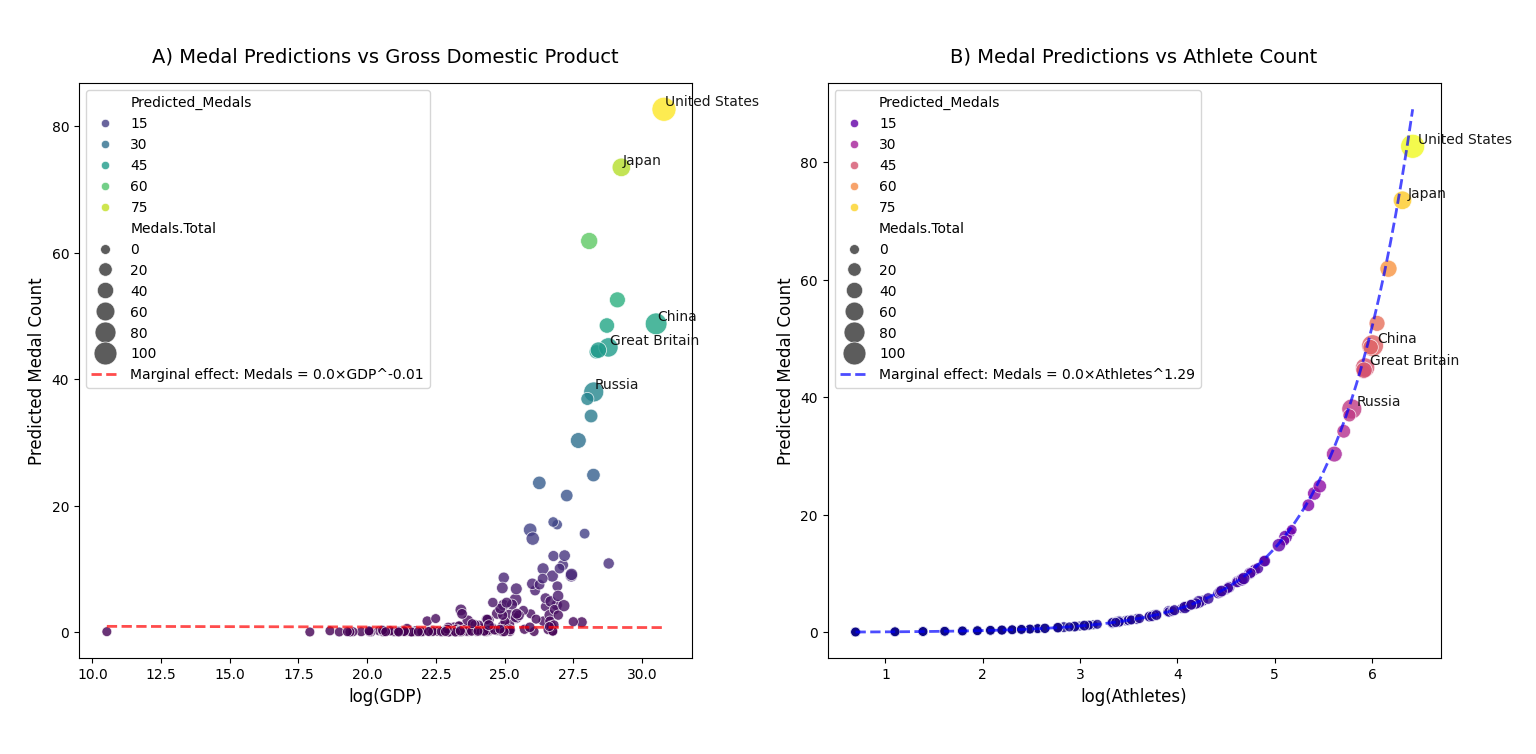
\includegraphics[width=0.8\textwidth]{model4.png}
\caption{GDP-Athletes Model Fitting Result}
\label{fig:model4}
\end{figure}

\begin{itemize}
    \item \textbf{Figure A}: The higher the GDP, the higher the predicted medal count, but the impact of GDP is not significant compared to the number of athletes.
    \item \textbf{Figure B}: The more athletes, the higher the predicted medal count, and the impact is significant.
\end{itemize}

The GDP-Athletes Model combines GDP and the number of athletes to predict the number of Olympic medals. Although GDP is theoretically related to the number of medals, its impact is not significant after controlling for the number of athletes. The number of athletes is a key variable for predicting the number of medals. For every 1\% increase in the number of athletes, the expected number of medals increases by about 1.29\%. Residual analysis shows that some countries with high GDP but low medal counts (such as Singapore and the United Arab Emirates) are overestimated, while some countries with low GDP but high medal counts (such as Jamaica and Georgia) are underestimated. This shows that the number of athletes is a more direct and effective indicator for predicting the number of Olympic medals, while the impact of GDP is more limited in practical applications.




% =============================================================================
% Conclusion
% =============================================================================
\section{Conclusion}
\label{sec:conclusion}

\subsection{Countries with Significant Forecast Anomalies}
\label{subsec:anomalies}

The residual diagnostics of the four zero-inflated negative binomial models all point to the same group of "systematically deviating countries." Based on the data from the 2021 Tokyo Olympics, they can be divided into two typical groups:

\paragraph{Countries that continue to be significantly overvalued}
Across all four model specifications, a consistent cohort of countries remains conspicuously over-predicted; their standardized residuals exceed $|2|$ in every iteration. 

\begin{itemize}
    \item \textbf{Argentina} appears in all four rounds: despite a sizeable athlete pool drawn from a medium-sized economy, medal yield is eroded by shrinking budgets and a fragmented training infrastructure. 
    
    \item \textbf{Chile} likewise registers in every list; high per-capita GDP notwithstanding, its summer-sport foundations are thin while winter programmes siphon off resources. 
    
    \item \textbf{South Africa} is flagged three times---ample population and GDP generate quantity without quality, as corruption in sport governance and declining athletics standards blunt returns. 
    
    \item \textbf{Algeria}, over-estimated four times, typifies the low-middle-income trap: once-dominant disciplines such as boxing and field events are in visible decline. 
    
    \item \textbf{Mexico} surfaces three times; its large demographic and economic mass is undercut by an Olympic budget persistently "siphoned" into professional football. 
    
    \item \textbf{Singapore}, the United Arab Emirates, Vietnam and Bangladesh appear two or three times each, confirming that neither exceptional wealth nor sheer population guarantees Olympic efficiency when domestic priorities divert investment elsewhere.
\end{itemize}

\paragraph{Countries that continue to be significantly undervalued}
Across all four model replications, a distinct group of nations persistently outperforms expectations, recording standardized residuals greater than $|2|$ in every instance. 

\begin{itemize}
    \item \textbf{Jamaica}, flagged in all four runs, leverages its global sprinting monopoly and an exceptionally efficient training system to convert a minuscule talent pool into disproportionate medal returns. 
    
    \item \textbf{Georgia}---population under four million---appears four times as well, capitalising on deeply rooted wrestling and weightlifting traditions reinforced by targeted state investment. 
    
    \item \textbf{San Marino}, one of the world's smallest sovereign states, is likewise listed four times; its microscopic size allows extraordinary per-capita Olympic expenditure concentrated on shooting and wrestling. 
    
    \item \textbf{Armenia}, similarly small and appearing four times, supplements a national boxing and wrestling system with substantial diaspora remittances earmarked for elite sport. 
    
    \item \textbf{Cuba} surfaces three times; despite a medium-sized economy constrained by sanctions, it sustains an in-depth specialisation in weightlifting that yields medals well beyond model forecasts. 
    
    \item \textbf{Bermuda}, Ukraine, Kenya and Ethiopia appear two or three times each, illustrating how limited GDP or population can be offset by outstanding, single-discipline advantages---triathlon for Bermuda, middle- and long-distance running for the East African pair, and residual Soviet-era expertise for Ukraine.
\end{itemize}

\subsection{Comparison of Indicator Selection}
\label{subsec:indicator_comparison}

\begin{enumerate}
    \item \textbf{Direct input indicators are better than macroeconomic indicators}
    
    When predicting the number of Olympic medals, the "actual number of participating athletes" as a direct input indicator has significantly better explanatory power and prediction accuracy than macro proxy variables such as GDP, population or HDI. The log-likelihood values of HDI-Athletes Model (HDI + number of athletes) and GDP-Athletes Model (GDP + number of athletes) are 66--142 units higher than those of HDI-Population Model (GDP + population) and GDP-Population Model (GDP + population), respectively, the AIC decreases by more than 130, and the pseudo $R^2$ increases by 15--18 percentage points, verifying the superiority of direct variables.
    
    \item \textbf{Double redundancy of GDP and population}
    
    When the model already includes the number of athletes, the logarithmic coefficients of GDP and population are not significant ($p>0.05$), and the sign direction is unstable (population is negative in GDP-Population Model). This shows that the two can only work by "indirectly affecting the scale of athletes" and have no additional marginal contribution to medal output.
    
    \item \textbf{"Per capita resource dilution effect"}
    
    The population variable is significantly negative in GDP-Population Model ($\beta=-0.250$), revealing the "demographic dividend paradox": if GDP does not grow synchronously with population, the population size will dilute the per capita Olympic investment and reduce the medal efficiency. This effect disappears in Models 2 and 4, further proving that the number of athletes has fully captured the nonlinear relationship between population and medals.
    
    \item \textbf{Residual stability test}
    
    The residual standard deviation (0.989--1.010) and the number of outliers (11) of the athlete number model are lower than those of the model without this variable (standard deviation 1.107--1.173, outliers 13--15), indicating that the athlete indicator can effectively suppress structural errors and improve the robustness of the model.
\end{enumerate}

% =============================================================================
% Bibliography
% =============================================================================
\bibliographystyle{abbrv}
\bibliography{literature}

\label{subsec:model_structure}

% =============================================================================
% Appendices
% =============================================================================
\appendix
\section*{Appendices}
\addcontentsline{toc}{section}{Appendices}

\section{Country Name Mapping}
\label{app:one}
[Standardization procedures for country names...]

\section{Additional Regression Outputs}
\label{app:two}
[Full statistical outputs for all models...]

\end{document}
